\scanpage{4}
transitivité -{}-{}-
\[R^i f_*\]
\uline{Suite spectrale de Leray}
\margin{....}

4°) Foncteurs fibres

Soit $\xi$ un pt géométrique de $X$
\[
\xi\xrightarrow{i}X,\quad \text{d'où foncteur fibre}
\]
\[
i^*:\widetilde X_{\mathrm{ét}}\longrightarrow\widetilde\xi_{\mathrm{ét}}\simeq(\operatorname{Ens})
\]
La famille des foncteurs fibres est \uline{conservative} : $u:F-G$ est un isom ssi les $u_{\bar x}:F_{\bar x}-G_{\bar x}$ le sont pour tt $x\in X$ d'où les cor. habituels.
\[
F_\xi=\underset{\substack{X'\text{ étale sur}\\X\text{ et pointé}\\\text{par }\xi}}{\unsure{\varinjlim}}F(X')
\]

5°) Localisation stricte
\diagram{\begin{tikzcd}
X'\arrow[d]&\xi\arrow[l]\arrow[dl]\\
X&
\end{tikzcd}}
\[
\underline{\mathcal O}_{X,\xi}\deleted{\unsure{\xi_X}}
=\underset{\substack{X'\text{ étale sur}\\X\text{ et }\xi\text{-pointé}}}{\underset{\longleftrightarrow}{\operatorname{Lim}}}
\Gamma(X',\mathcal O_{X'})
\]
\margin{anneaux stricts locaux ou \unsure{strict.t local} i.e.\ \deleted{\unsure{hensélien et}} hensélien et à corps rés. sép. clos}
\[
\bar X^{\unsure{\xi}}=\operatorname{Spec}\mathcal O_{X,\xi}
\]
\[
F_\xi=\Gamma(\bar X,\unsure{\widetilde F}_{\bar X})
\]

6°) Application aux fibres des $R^qf_*(F)$, pour $f$ qu. cpt. et qu. sép.

\margin{\uline{NB} 5° et 6° \unsure{n'a} pas vraiment d'analogue complet dans le cas des espaces top. ordinaires .....}
\figure{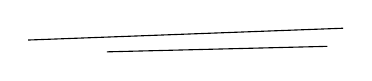
\begin{tikzpicture}\draw (0,0)--(4,.15);\draw (1,-.15)--(3.8,-.08);\end{tikzpicture}}

7°) \uuline{Théorème fondamental} Soit $f:X-Y$ un morphisme propre, $F$ faisceau \uline{de torsion} sur $X$, alors la formation des $R^{\unsure{i|q}}f_*(F)$
\mspage{3}
